%%%%%%%%%%%%%%%%%%don't forget if needed %%%%%%%%%%%%%%%%%%%%%
%\section[toc version]{title version%
%              \sectionmark{head version}}
%\sectionmark{head version}
%%%%%%%%%%%%%%%%%%%%%%%%%%%%%%%%%%%%%%%%%%%%%%%%%%%%%%%%%%%%%%
\def\titcourt{Navier-Stokes-Boussinesq and enthalpy-porosity models}
\def\titlong{Navier-Stokes-Boussinesq and enthalpy-porosity models}
%%%%%%%%%%%%%%%%%%%%%%%%%%%%%%%%%%%%%%%%%%%%%%%%%%%%%%%%%%%%%%%%
\chapter[\titlong]{\titlong%
              \chaptermark{\titcourt}}
\chaptermark{\titcourt}
\label{chap-NSB}
%%%%%%%%%%%%%%%%%%%%%%%%%%%%%%%%%%%%%%%%%%%%%%%%%%%%%%%%%%%%%%%%
%%%%%%%%%%%%%%%%%%%%%%%%%%%%%%%%%%%%%%%%%%%%%%%%%%%%%%%%%%%%%%%%

%\section{Governing equations} \label{sec-gov-eq}
%%%%%%%%%%%%%%%%%%%%%%%%%%%%

We consider a solid-liquid system placed in a 2D or 3D domain $\Omega$ of characteristic length $L_{ref}$. 
In the following, subscripts $s$ and $l$ will refer to the solid and liquid phases, respectively. 

The single domain approach, using the same system of equations in both phases, is described first in detail.
The model is based on the Navier-Stokes equations with Boussinesq approximation, which is the natural description of the fluid flow with natural convection. 
A penalty term is added to the momentum equations to bring the velocity to zero inside the solid region. 
For the energy conservation equation, an enthalpy-porosity method is used to model the phase change process. %The single-domain model is  in detail in the following sections.

\section{Enthalpy-porosity model}

The phase change process is modeled using an enthalpy method with temperature-based formulation  \citep{voller1987pcm,Cao1989,Cao1990}. We start from the classical energy equation:
\begin{equation}
\label{eq-energie}
   \frac{\partial (\rho h)}{\partial t_{\varphi}} + \nabla \cdot(\rho h \vec{U}) - \nabla \cdot (k \nabla T) = 0,
\end{equation}

\noindent where $t_{\varphi}$ is the physical time, $h$ the enthalpy, $\rho$ the density, $\vec{U}$  the velocity vector, $T$ the temperature and $k$ the thermal conductivity. 
The total enthalpy $h$ is transformed as the sum of the sensible heat and the latent heat:
\begin{equation}
\label{eq-enth-model}
  h = h_{sen} + h_{lat} = c ( T + s(T) ),
\end{equation} 

\noindent with $c$ the local specific heat. The function $s$ is introduced to model the jump of the enthalpy during the solid-liquid transition.  For pure materials, $s$ is theoretically  a Heaviside step function depending on the temperature: it takes the zero value in the solid region and a large value in the liquid, equal to $h_{sl}/c_l$, with $h_{sl}$ the latent heat of fusion. 

\noindent If the phase-change is assumed to occur within a mushy zone defined by a small temperature interval $  T \in [T_f - T_\varepsilon, T_f + T_\varepsilon] $ around the temperature of fusion $T_f$, a model for $s(T)$ is necessary. 
Linear  \citep{voller1987pcm,Wang2010} or more smooth functions \citep{dan-2014-JCP} can be used to regularize $s(T)$ and thus model the jump of material properties from solid to liquid.  
In the current work we use a regularization of all step-functions (latent heat source, specific heat, thermal diffusivity or conductivity) by a continuous and differentiable hyperbolic-tangent function suggested by \cite{dan-2014-JCP}.

\noindent We assume moreover that the undercooling phenomenon is negligible during the solidification stage (see also \cite{wang2010numerical,kowalewski2004phase}).
The solid-liquid interface is identified through the isoline $T=T_f$, while the Gibbs-Thomson effect due to the surface energy of the solid-liquid interface is assumed to be negligible.% in our simulations.

\noindent Equation \eqref{eq-energie} can be further simplified by considering the following assumptions: 
\begin{enumerate}[label=(\roman*)]
\item the density difference between solid and liquid phases is negligible, \ie $\rho_l=\rho_s=\rho$ is constant. 
We note however that this is not strictly true for all substances, but it serves here as a convenient simplification,
\item the regularization zone is narrow and the velocity inside this zone is negligible. 
\end{enumerate}
Consequently, the final expression of the energy equation is obtained by combining Eqs. \eqref{eq-enth-model}  and \eqref{eq-energie} and  neglecting the convection term $\nabla \cdot ( c s \vec{U})$\footnote{In the liquid phase, $\nabla \cdot ( c s \vec{U})  = h_{sl} \nabla \cdot  \vec{U}=0$; in the solid phase, $s=0$; in the regularization (mushy) region, it is assumed that $\vec{U}=0.$}:\\

\begin{equation}\label{eq-energie-enth-model}
\frac{\partial \left(c T\right)}{\partial t_{\varphi}} + \nabla \cdot\left( c T \vec{U}\right) -
\nabla \cdot\left( \frac{k}{\rho} \nabla T \right) +  \frac{\partial \left(c s\right)}{\partial t_{\varphi}}  = 0.
\end{equation}

\section{Navier-Stokes equations with Boussinesq approximation}

The natural convection in the liquid part of the system is modeled using the incompressible Navier-Stokes equations, with  Boussinesq approximation for buoyancy effects. To make this model valid for both liquid and solid phases, the momentum equation is modified as following:
\begin{equation}\label{eq-momentum-conserv-1}
\frac{\partial \vec{U}}{\partial t_{\varphi}} +   {(\vec{U}\cdot\nabla ) \vec{U}} + \frac{1}{\rho}\nabla P - \frac{\mu_{l}}{\rho}   {\nabla^2 \vec{U}} 
+ \rho g \vec{e}_y= A(T) \vec{U},
\end{equation}

\noindent where $P$ denotes the pressure and $\mu_{l}$ the dynamic viscosity of the liquid (assumed to be constant).  

\noindent The penalty term $A(T) \vec{U}$ is artificially introduced in Eq. \eqref{eq-momentum-conserv-1} to extend this equation in the solid phase, where the velocity, pressure, viscosity and Boussinesq force are meaningless.  Consequently, $A(T)$  is modelled to vanish in the liquid, where the Navier-Stokes-Boussinesq momentum equation is recovered. A large value of $A(T)$ is imposed in the solid, reducing the momentum Eq. \eqref{eq-momentum-conserv-1}  to $A(T) \vec{U}=0$, equivalent to $\vec{U}=0$. 
The exact expression for $A$ will be given in the next section.

\noindent The density is assumed to be constant everywhere except in the body force term $\rho g$ of the $\vec e_y$ momentum Eq. \eqref{eq-momentum-conserv-1}.
Under the assumption of a small variation of the density and the temperature, the Boussinesq approximation allows to linearize the density as follows:
\begin{equation}
   \rho = \rho_{ref} (1 - \beta (T-T_{ref})),
\end{equation}

\noindent with $\beta = - (1/\rho_{ref}) (\partial \rho / \partial T)$ the thermal expansion coefficient and $(\rho_{ref},T_{ref})$ a reference state.
It is worth noting that this approximation is valid for $\beta (T - T_{ref})$ considerably smaller than the unity.
Therefore, the momentum equation can be written as
\begin{equation}\label{eq-momentum-conserv}
  \frac{\partial \vec{U}}{\partial t_{\varphi}} +   {(\vec{U}\cdot\nabla ) \vec{U}} + \nabla p - \nu_{l}  {\nabla^2 \vec{U}} 
- f_B(T) \vec{e}_y= A(T) \vec{U},
\end{equation}

\noindent where  $\nu_l = \mu_l/\rho$ is the kinematic viscosity,  $p = (P + \rho_{ref} g y)/ \rho_{ref}$ includes the hydrostatic pressure $\rho_{ref} g y$ and $f_B(T) = g \beta (T-T_{ref})$ denotes the buoyancy force.

Finally, the conservation of mass in the liquid phase is expressed by the continuity equation in the frame of incompressible fluids:
\begin{equation}\label{eq-mass-conserv}
\nabla \cdot \vec{U} = 0.
\end{equation} 

\noindent The final system of equations for the single-domain approach is thus: 

\begin{eqnarray} 
	\nabla \cdot \vec{U} &=& 0, \\
	\frac{\partial \vec{U}}{\partial t_{\varphi}} +   {(\vec{U}\cdot\nabla ) \vec{U}} + \nabla p - \nu_{l}  {\nabla^2 \vec{U}} 
- f_B(T) \vec{e}_y - A(T) \vec{U} & = & 0, \\
	\frac{\partial \left(c T\right)}{\partial t_{\varphi}} + \nabla \cdot\left( c T \vec{U}\right) -
\nabla \cdot\left( \frac{k}{\rho} \nabla T \right) +  \frac{\partial \left(c s\right)}{\partial t_{\varphi}}  &=& 0.
\end{eqnarray}


\section{Dimensionless system of equations for the single-domain approach}\label{sec-eq-scaling}

It is convenient to numerically solve a dimensionless form of the previous equations.
After choosing a reference length $L_{ref}$ (usually the height of the cavity when a rectangular domain is considered) and a reference state $(\rho, V_{ref}, T_{ref})$, we can define the following scaling for the space, velocity, temperature and time variables:
\begin{equation}\label{eq-adim}
\vec{x} = \frac{\vec{X}}{L_{ref}} \, , \,  \vec{u} = \frac{\vec{U}}{V_{ref}} \, , \,  \theta = \frac{T-T_{ref}}{\delta T} \, , \,  t = \frac{V_{ref}}{L_{ref}} \, t_{\varphi}.
\end{equation}

\noindent $T_{ref}$ is the reference temperature and in most cases $T_{ref} = T_f$ (the temperature of fusion), unless otherwise specified.
Consequently, the non-dimensional temperature of fusion is set to $\theta_f = 0$.
Temperature difference  $\delta T$, defines a temperature scale, that will be set differently for melting and solidification cases.
$\delta T$ is considered as the representative temperature scale  for the natural convection onset in the liquid region. 
For the classical natural convection problem without phase-change, $\delta T$ is generally defined as $\delta T=T_{h}-T_{c}$ since the flow in the fluid is driven by the temperature difference between the "hot" and the "cold" temperature.
However, for the melting PCM, the convection is driven by the temperature difference $\delta T=T_{h}-T_{f}$, with $T_f$ the temperature of fusion.
As far as the solidification process is concerned, a distinct discussion will be provided in Chapter \ref{chap-SOLIDIFICATION}. 

The dimensionless system of equations to be solved in both liquid and solid regions can be finally written as:
\begin{eqnarray}
\nabla\cdot \vec{u}&=&0, \label{eq-qmvt} \\ \vspace{0.2cm}
 \frac{\partial \vec{u}}{\partial t} + {(\vec{u}\cdot\nabla) \vec{u}} +\nabla p -\frac{1}{\Rey}{\nabla^2 \vec{u}} 
 - f_B(\theta)\, \vec{e}_y - A(\theta) \vec{u}&=&0, \label{eq-qmvt-2} \\ \vspace{0.2cm}
 \frac{\partial \left(C \theta\right)}{\partial t} + \nabla \cdot\left( C \theta \vec{u}\right) -
 \nabla \cdot\left( \frac{K}{\Rey \Prd} \nabla \theta \right) +  \frac{\partial \left(C S\right)}{\partial t}  &=& 0. \label{eq-energ} 
\end{eqnarray}

\noindent The linearised Boussinesq buoyancy force ($f_B$), the Reynolds ($Re$) and Prandtl ($\Prd$) numbers are defined as
\begin{equation}\label{eq-RePr}
f_B(\theta) = \frac{\Ray}{\Prd \Rey^2} \theta, \quad \Rey = \frac{\rho V_{ref} L_{ref}}{\mu_l}=  \frac{V_{ref} L_{ref}}{\nu_l} , \quad \Prd = \frac{\nu_l}{\alpha_l},
\end{equation}
with $\alpha = k/(\rho c)$  the thermal diffusivity. In the expression of $f_B$, the Rayleigh number of the flow is defined as
\begin{equation}
\label{eq-Rayleigh}
\Ray = \frac{g \beta L_{ref}^3 \delta T}{\nu_l \alpha_l},
\end{equation}
with $\beta$ the thermal expansion coefficient and $g$ the gravitational acceleration.

\noindent If previous non-dimensional numbers are pertinent only in the liquid phase, the non-dimensional conductivity and specific heat are  defined in both phases
\begin{equation}\label{eq-adimKC}
K(\theta)= \frac{k}{k_l} =\left\{
\begin{matrix}
1, & \theta \geq \theta_f ,\\
k_s/k_l, & \theta < \theta_f .\\
\end{matrix}
\right.
, \,  \, C(\theta) = \frac{c}{c_l}=\left\{
\begin{matrix}
1, & \theta \geq \theta_f ,\\
c_s/c_l, & \theta < \theta_f .\\
\end{matrix}
\right.
\end{equation}

\noindent The non-dimensional function $S = s/s_l$ in the energy Eq. \eqref{eq-energ} takes a similar non-dimensional form:
\begin{equation}\label{eq-adimS}
S(\theta)= \frac{s}{s_l} =\left\{
\begin{array}{rl} \vspace{0.2cm}
\ds \frac{h_{sl}/c_l}{\delta T} = \frac{1}{Ste}, & \theta \geq \theta_f ,\\
0, & \theta < \theta_f,\\
\end{array}
\right.
\end{equation}

\noindent with $Ste$ the Stefan number.

\noindent Discontinuous step-functions defined in Eqs. \eqref{eq-adimKC}  and \eqref{eq-adimS} are replaced by continuous and differentiable hyperbolic-tangent functions, generically defined for all $\theta$ by the formula \citep{dan-2014-JCP}
\begin{equation}
F(\theta; a_r, \theta_r, R_r) = f_l + \frac{f_s-f_l}{2}\left\{
1 + \tanh\left( a_r \left(\frac{\theta_r-\theta}{R_r}\right)\right)
\right\},
\label{eq-smooth}
\end{equation}

\noindent where $f_l, f_s$ are the imposed values in the liquid and solid phases, $a_r$ a smoothing  parameter, $\theta_r$ the central value (around which we regularize), and $R_r$ the smoothing radius. For example, we use for the non-dimensional source term in Eq. \eqref{eq-energ} the following regularisation over the artificial mushy region $\theta \in [-\varepsilon, \varepsilon]$:
\begin{equation}
S(\theta) = \frac{1}{\Ste} - \frac{1}{2\,\Ste}\left\{
1 + \tanh\left(\frac{\theta_s-\theta}{R_s}\right)
\right\},
\label{eq-Stanh}
\end{equation} 

\noindent with $\theta_s=\theta_f=0$ and $R_s=\varepsilon$ for the melting case. 

Finally, the penalty term in the momentum Eq. \eqref{eq-qmvt-2} is derived from the Darcy's law, by modeling the fluid flow within the mushy region as a flow through a porous medium.
In fact, the Darcy's law states that the velocity of flow in porous medium is proportional to the pressure gradient:

\begin{equation}
	\vec u = - \frac{\zeta^*}{\mu} \vec \nabla p.
\end{equation}

\noindent where $\zeta^*$ is the permeability, which is a function of the porosity.
As the porosity decreases, the permeability (and the velocity) also decreases, down to the limiting value of zero when the mushy zone becomes completely solid.
This behavior can be accounted in a numerical model by adding a source term $A \vec u$ in the momentum equation.
The well-known equation derived from the Darcy law is the Carman-Kozeny model:

\begin{equation} \label{ck eq}
	\nabla p = - \frac{\CKC (1 - \lambda)^2}{\lambda^3} \vec u.
\end{equation}

\noindent Consequently, $A$ takes the form \citep{Belhamadia2012,kheirabadi2015effect}
\begin{equation}\label{eq-CK}
A(\theta) = -\frac{\CKC (1 - L_f(\theta))^2}{L_f(\theta)^3 + b}, 
\end{equation}

\noindent where $L_f(\theta)$ is the local liquid fraction, which is  $1$ in the fluid region and  $0$ in the solid. $L_f$ is regularized inside the artificial  mushy-region using a hyperbolic-tangent similar to Eq. \eqref{eq-Stanh}.
The Carman-Kozeny constant $\CKC$ is set to a  large value (as discussed below) and  the constant $b=10^{-6}$ is introduced to avoid divisions by zero.

\section{Boundary layer approximation and scale analysis} \label{sec-bound-scal-anal}
Regardless to the practical use of PCM (energy storage, or for building insulation, or for other purposes), one would necessarily assess the heat transfer during the phase-change process.
It was extensively proven that the convective heat transfer plays a significant role during the melting stage.
Therefore, before solving numerically Eqs. \eqref{eq-qmvt} - \eqref{eq-energ}, we first rely on a scale analysis to predict theoretically the fluid flow and heat transfer patterns that can develop in the fluid part.
The idea behind the scaling analysis is to identify the proper scales of the phenomenon, in order to understand the evolution of the heat transfer and the melting rate.
We consider only the liquid phase without phase-change, inside a two-dimensional enclosure of height H filled with Newtonian fluid, differentially heated from the vertical walls and insulated at the horizontal walls.
A homogeneous Dirichlet boundary condition is prescribed for the velocity. 
%The purpose is to give some insight in the main orders of magnitude for heat transfer in natural convection.
One may refer to the book by \cite{bejan2013convection} for a more detailed presentation.

Since no external force is applied to our system, the fluid flow is mainly driven by natural convection, induced by the temperature difference from the vertical walls.
%It is well-known from the foregoing boundary conditions that the fluid layer situated close to the vertical walls stuck to the wall and are motionless.
The heat transfer through the fluid layer immediately adjacent to the wall is assumed to be driven by pure conduction.
We therefore define the average Nusselt number to quantify the heat transfer rate at the hot wall (placed at $x=0$):
\begin{equation}\label{eq-def-Nu}
   \mathcal{N}\!u = - \int_0^1 \left. \frac{\partial \theta}{\partial x} \right |_{x=0} dy.
\end{equation}

When a steady state could be reached, the fluid near each sidewall is characterized by two boundary layers: a thermal boundary layer of thickness $\delta_{\theta}$ and a viscous boundary layer of thickness $\delta_\nu$.
The boundary layer approximation assumes that the flow and the energy transfer are restricted predominantly to the boundary layer region.
%This theory was proposed first by Prandtl in 1904 and validated later by many experimental and numerical studies.
The main consequences of the boundary layer approximation are that:
\begin{enumerate}[label=(\roman*)]
\item the normal part of the momentum equation has a negligible importance,
\item the downstream diffusion term in the momentum and energy equations are neglected in comparison with the normal diffusion terms,
\item the pressure distribution is purely hydrostatic,
\item the thermal and the viscous boundary layer thickness are related by following expression: $\delta_\nu/\delta_\theta = o \left(\Prd^{1/2} \right)$.
\end{enumerate}

\noindent Scaling laws developed by \cite{bejan2013convection}, presented in Fig. \ref{fig:min-size-bnd}, relying on boundary layer approximation reads

\begin{equation} \label{eq-bnd-layer-T}
   \delta_T \sim \left\{
   \begin{array}{ll}
   H \Ray^{-1/4} &	 \mbox{if }  \Prd \gg 1,\\
   H \Prd^{-1/4} \Ray^{-1/4} &   \mbox{if } \Prd \ll 1.
   \end{array}
   \right.
\end{equation}

\noindent Since the Nusselt number from Eq. \eqref{eq-def-Nu} scales as $H/\delta_\theta$, \cite{bejan2013convection} have suggested the following $\mathcal{N}\!u - \Ray$ correlations:

\begin{equation} \label{eq-Nu}
   \mathcal{N}\!u \sim \left\{
   \begin{array}{ll}
   \Ray^{1/4} &	 \mbox{if }  \Prd \gg 1,\\
   \Prd^{1/4} Ra^{1/4} &   \mbox{if } \Prd \ll 1.
   \end{array}
   \right.
\end{equation}

\begin{figure}
	\begin{center}
		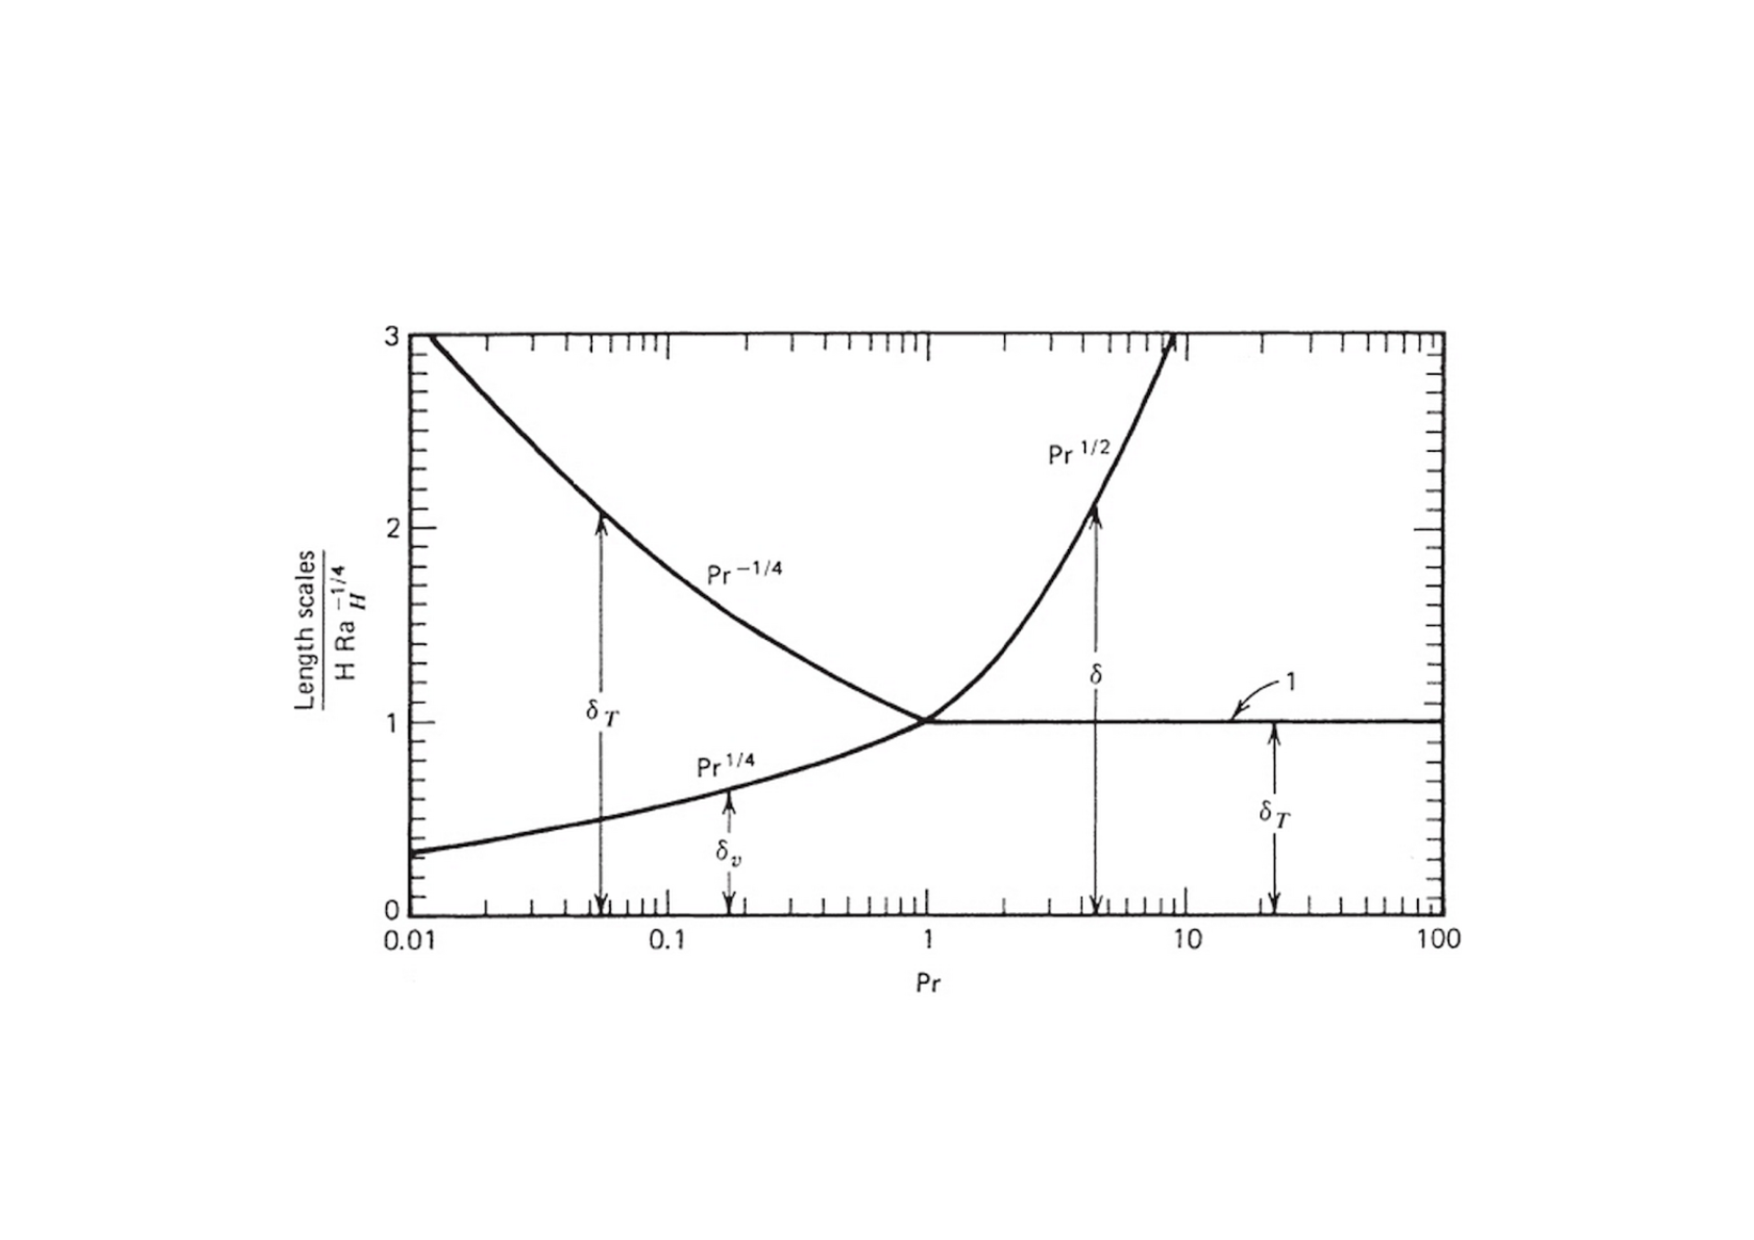
\includegraphics[width=.9\textwidth]{\figpath/Fig_cap_melting/thermal_bnd}
	\end{center}
	\caption{Thermal and viscous boundary layer thickness function of the Prandtl number \citep{bejan2013convection}.}
	\label{fig:min-size-bnd}
\end{figure}

\noindent Correlation \eqref{eq-bnd-layer-T} is useful to estimate the scale of the boundary layer for mesh adaptivity, since the minimum edge length should allow to capture the smaller length scale in the flow.
For low-Prandtl fluid, the viscous boundary layer is finer than the thermal boundary layer, and conversely, the thermal boundary layer is finer for high-Prandtl fluid.



